%%%%%%%%%%%%%%%%%%%%%%%%%%%%%%%%%%%%%%%%%
% Short Sectioned Assignment
% LaTeX Template
% Version 1.0 (5/5/12)
%
% This template has been downloaded from:
% http://www.LaTeXTemplates.com
%
% Original author:
% Frits Wenneker (http://www.howtotex.com)
%
% License:
% CC BY-NC-SA 3.0 (http://creativecommons.org/licenses/by-nc-sa/3.0/)
%
%%%%%%%%%%%%%%%%%%%%%%%%%%%%%%%%%%%%%%%%%

%----------------------------------------------------------------------------------------
%	PACKAGES AND OTHER DOCUMENT CONFIGURATIONS
%----------------------------------------------------------------------------------------

\documentclass[paper=a4, fontsize=11pt]{scrartcl} % A4 paper and 11pt font size

\usepackage{multicol}
\usepackage[T1]{fontenc} % Use 8-bit encoding that has 256 glyphs
\usepackage{fourier} % Use the Adobe Utopia font for the document - comment this line to return to the LaTeX default
\usepackage[english]{babel} % English language/hyphenation
\usepackage{amsfonts,amssymb,latexsym,amsmath,amsthm,amscd}

\usepackage[left=2cm,right=2cm,top=3cm,bottom=3cm]{geometry}
\usepackage{sectsty} % Allows customizing section commands
\allsectionsfont{\centering \normalfont\scshape} % Make all sections centered, the default font and small caps

\usepackage{fancyhdr} % Custom headers and footers
\pagestyle{fancyplain} % Makes all pages in the document conform to the custom headers and footers
\fancyhead{} % No page header - if you want one, create it in the same way as the footers below
\fancyfoot[L]{} % Empty left footer
\fancyfoot[C]{} % Empty center footer
\fancyfoot[R]{\thepage} % Page numbering for right footer
\renewcommand{\headrulewidth}{0pt} % Remove header underlines
\renewcommand{\footrulewidth}{0pt} % Remove footer underlines
\setlength{\headheight}{13.6pt} % Customize the height of the header

\numberwithin{equation}{section} % Number equations within sections (i.e. 1.1, 1.2, 2.1, 2.2 instead of 1, 2, 3, 4)
\numberwithin{figure}{section} % Number figures within sections (i.e. 1.1, 1.2, 2.1, 2.2 instead of 1, 2, 3, 4)
\numberwithin{table}{section} % Number tables within sections (i.e. 1.1, 1.2, 2.1, 2.2 instead of 1, 2, 3, 4)

\setlength\parindent{0pt} % Removes all indentation from paragraphs - comment this line for an assignment with lots of text


%%%%%%%%%% Commands
\usepackage[all]{xy}
\xyoption{arc}

\usepackage{graphicx}
\usepackage{cmap}

%Blackboard Letters
\newcommand{\bbQ}{\mathbb{Q}}
\newcommand{\bbI}{\mathbb{I}}
\newcommand{\bbL}{\mathbb{L}}
\newcommand{\bbF}{\mathbb{F}}
\newcommand{\bbC}{\mathbb{C}}
\newcommand{\bbD}{\mathbb{D}}
\newcommand{\bbZ}{\mathbb{Z}}
\newcommand{\bbP}{\mathbb{P}}
\newcommand{\bbA}{\mathbb{A}}
\newcommand{\bbB}{\mathbb{B}}
\newcommand{\bbR}{\mathbb{R}}
\newcommand{\bbG}{\mathbb{G}}
\newcommand{\bbE}{\mathbb{E}}
\newcommand{\bbH}{\mathbb{H}}
\newcommand{\bbN}{\mathbb{N}}
\newcommand{\bbT}{\mathbb{T}}
\newcommand{\bbW}{\mathbb{W}}
\newcommand{\bbV}{\mathbb{V}}

%Bold Letters 
\newcommand{\bQ}{\mathbf{Q}}
\newcommand{\bF}{\mathbf{F}}
\newcommand{\bC}{\mathbf{C}}
\newcommand{\bJ}{\mathbf{J}}
\newcommand{\bZ}{\mathbf{Z}}
\newcommand{\bP}{\mathbf{P}}
\newcommand{\bA}{\mathbf{A}}
\newcommand{\bR}{\mathbf{R}}
\newcommand{\bG}{\mathbf{G}}
\newcommand{\bE}{\mathbf{E}}
\newcommand{\bH}{\mathbf{H}}
\newcommand{\bN}{\mathbf{N}}

%(for Q,R,N,C,...)
\renewcommand{\AA}{\bbA}
\newcommand{\BB}{\bbB}
\newcommand{\DD}{\bbD}
\newcommand{\QQ}{\bbQ}
\newcommand{\II}{\bbI}
\newcommand{\WW}{\bbW}
\newcommand{\RR}{\bbR}
\newcommand{\CC}{\bbC}
\newcommand{\VV}{\bbV}
\newcommand{\FF}{\bbF}
\newcommand{\HH}{\bbH}
\newcommand{\ZZ}{\bbZ}
\newcommand{\NN}{\bbN}
\newcommand{\PP}{\bbP}

\newcommand{\Qbar}{\overline{\QQ}}

%Caligraphic (Sheaves...)
\newcommand{\cA}{\mathcal{A}}
\newcommand{\cB}{\mathcal{B}}
\newcommand{\cC}{\mathcal{C}}
\newcommand{\cD}{\mathcal{D}}
\newcommand{\cO}{\mathcal{O}}
\newcommand{\cF}{\mathcal{F}}
\newcommand{\cG}{\mathcal{G}}
\newcommand{\cI}{\mathcal{I}}
\newcommand{\cJ}{\mathcal{J}}
\newcommand{\cL}{\mathcal{L}}
\newcommand{\cH}{\mathcal{H}}
\newcommand{\chh}{\mathcal{h}}
\newcommand{\cR}{\mathcal{R}}
\newcommand{\cM}{\mathcal{M}}
\newcommand{\cN}{\mathcal{N}}
\newcommand{\cE}{\mathcal{E}}
\newcommand{\cP}{\mathcal{P}}
\newcommand{\cT}{\mathcal{T}}
\newcommand{\cU}{\mathcal{U}}
\newcommand{\cV}{\mathcal{V}}
\newcommand{\cW}{\mathcal{W}}
\newcommand{\cZ}{\mathcal{Z}}

\newcommand{\cHom}{\operatorname{\mathcal{H}om}}
\newcommand{\shomega}{\underline{\omega}}

%Category names
\newcommand{\AbGrp}{\textbf{Ab}}
\newcommand{\Ab}{\AbGrp}
\newcommand{\Sheaves}{\textbf{Sheaves}}
\newcommand{\Rings}{\textbf{Rings}}
\newcommand{\Mod}{\textbf{Mod}}
\newcommand{\Sh}{\textbf{Sh}}
\newcommand{\Sch}{\textbf{Sch}}
\newcommand{\Sets}{\textbf{Sets}}
\newcommand{\Mot}{\textbf{Mot}}

%Fraktor letters, eg naming ideals

\newcommand{\fA}{\mathfrak A}
\newcommand{\fR}{\mathfrak R}
\newcommand{\fp}{\mathfrak p}
\newcommand{\fq}{\mathfrak q}
\newcommand{\fP}{\mathfrak P}
\newcommand{\fQ}{\mathfrak Q}
\newcommand{\fa}{\mathfrak a}
\newcommand{\fb}{\mathfrak b}
\newcommand{\fc}{\mathfrak c}
\newcommand{\fd}{\mathfrak d}
\newcommand{\fm}{\mathfrak m}
\newcommand{\fn}{\mathfrak n}
\newcommand{\fo}{\mathfrak o}
\newcommand{\fS}{\mathfrak S}
\newcommand{\fN}{\mathfrak N}
\newcommand{\fU}{\mathfrak U}
\newcommand{\fX}{\mathfrak X}
\newcommand{\fY}{\mathfrak Y}

\def\wh{\widehat}

%Some common math operators
\DeclareMathOperator{\order}{ord}
\DeclareMathOperator{\Inf}{Inf}
\DeclareMathOperator{\Cris}{Cris}
% \DeclareMathOperator{\Sh}{Sh}
\DeclareMathOperator{\val}{val}
\DeclareMathOperator{\Ram}{Ram}
\DeclareMathOperator{\Stab}{Stab}
\DeclareMathOperator{\St}{St}
\DeclareMathOperator{\sgn}{sgn}
\DeclareMathOperator{\rk}{rk}
\DeclareMathOperator{\cork}{cork}
\DeclareMathOperator{\lcm}{lcm}
\DeclareMathOperator{\Gal}{Gal}
\DeclareMathOperator{\Spec}{Spec}
\DeclareMathOperator{\Max}{Max}
\DeclareMathOperator{\Sp}{Sp}
\DeclareMathOperator{\Mp}{Mp}
\DeclareMathOperator{\Spf}{Spf}
\DeclareMathOperator{\Proj}{Proj}
\DeclareMathOperator{\Jacobson}{\mathfrak J}
\DeclareMathOperator{\Nilradical}{\mathfrak N}
\DeclareMathOperator{\rad}{\mathfrak{rad}}
\DeclareMathOperator{\Hom}{Hom}
\DeclareMathOperator{\End}{End}
\DeclareMathOperator{\Aut}{Aut}
\DeclareMathOperator{\Isom}{Isom}
\DeclareMathOperator{\car}{char}
\DeclareMathOperator{\gl}{GL}
\DeclareMathOperator{\GL}{GL}
\DeclareMathOperator{\PGL}{PGL}
\DeclareMathOperator{\tr}{Tr}
\DeclareMathOperator{\disc}{disc}
\DeclareMathOperator{\discrd}{discrd}
\DeclareMathOperator{\supp}{Supp}
\DeclareMathOperator{\Div}{Div}
\DeclareMathOperator{\Pic}{Pic}
\DeclareMathOperator{\divv}{div}
%\DeclareMathOperator{\ord}{ord}
\DeclareMathOperator{\res}{Res}
\DeclareMathOperator{\coker}{coker}
\DeclareMathOperator{\img}{img}
\DeclareMathOperator{\Tate}{Tate}
\DeclareMathOperator{\gr}{gr}
\DeclareMathOperator{\Tot}{Tot}
\DeclareMathOperator{\Tor}{Tor}
\DeclareMathOperator{\sym}{Sym}
\DeclareMathOperator{\ev}{ev}
\DeclareMathOperator{\Symm}{Symm}
\DeclareMathOperator{\Ann}{Ann}
\DeclareMathOperator{\length}{length}
\DeclareMathOperator{\dlog}{dlog}
\DeclareMathOperator{\chow}{CH}
\DeclareMathOperator{\cl}{cl}
\DeclareMathOperator{\Cl}{Cl}
\DeclareMathOperator{\AJ}{AJ}
\DeclareMathOperator{\Ext}{Ext}
\DeclareMathOperator{\Sym}{Sym}
\DeclareMathOperator{\Nm}{Nm}
\DeclareMathOperator{\nrd}{Nrd}
\DeclareMathOperator{\trd}{trd}
\DeclareMathOperator{\Corr}{Corr}
\DeclareMathOperator{\pr}{pr}
\DeclareMathOperator{\SL}{SL}
\DeclareMathOperator{\PSL}{PSL}
\DeclareMathOperator{\SO}{SO}
\DeclareMathOperator{\SU}{SU}
\DeclareMathOperator{\Graph}{Graph}
\DeclareMathOperator{\Fil}{Fil}
\DeclareMathOperator{\red}{red}
\DeclareMathOperator{\MF}{MF}
\DeclareMathOperator{\Rep}{Rep}
\DeclareMathOperator{\Reg}{Reg}
\DeclareMathOperator{\Frac}{Frac}
\DeclareMathOperator{\Dst}{D_{\st}}
\DeclareMathOperator{\Vst}{V_{\st}}
\DeclareMathOperator{\NS}{NS}
\DeclareMathOperator{\ad}{ad}
\DeclareMathOperator{\stab}{stab}
\DeclareMathOperator{\Gr}{Gr}
\DeclareMathOperator{\Frob}{Frob}
\DeclareMathOperator{\cond}{cond}
\DeclareMathOperator{\Sel}{Sel}
\DeclareMathOperator{\Ind}{Ind}
\DeclareMathOperator{\cInd}{c-Ind}
\def\det{\operatorname{det}}
\DeclareMathOperator{\diag}{diag}
\DeclareMathOperator{\Alb}{Alb}
\DeclareMathOperator{\Jet}{Jet}
\DeclareMathOperator{\Lie}{Lie}
\DeclareMathOperator{\LIM}{LIM}

% Some common abreviations
\newcommand{\lto}{\longrightarrow}
\newcommand{\dfn}{\ensuremath{{:=}}}
\newcommand{\nfd}{\ensuremath{{=:}}}
\newcommand{\surjects}{\twoheadrightarrow}
\newcommand{\injects}{\hookrightarrow}
\newcommand{\id}{\ensuremath \text{Id}}
\newcommand{\tns}[1][]{\otimes_{\!#1}}
\newcommand{\mtx}[4]{\left(\begin{matrix}#1&#2\\#3&#4\end{matrix}\right)}
\newcommand{\mat}[1]{\left(\begin{matrix}#1\end{matrix}\right)}
\newcommand{\smat}[1]{\left(\begin{smallmatrix}#1\end{smallmatrix}\right)}
\newcommand{\smtx}[4]{\left(\begin{smallmatrix}#1&#2\\#3&#4\end{smallmatrix}\right)}
\newcommand{\slz}{\operatorname{SL}_2(\ZZ)}

\def\sumprime{\mathop{\sum{\raise3pt\hbox{${}'$}}}} %Copied from somewhere else...
\def\prodprime{\mathop{\prod{\raise3pt\hbox{${}'$}}}} %Copied from somewhere else...

\newcommand{\et}{{\text{et}}}
\newcommand{\dR}{{\text{dR}}}
\newcommand{\cont}{{\text{cont}}}
\newcommand{\cris}{{\text{cris}}}
\newcommand{\Het}{H_\et}
\newcommand{\Hdr}{H_\dR}
\newcommand{\Hcris}{H_\cris}
\newcommand{\Bcris}{B_\cris}
\newcommand{\Dcris}{D_\cris}
\newcommand{\Vcris}{V_\cris}
\newcommand{\cHdr}{\cH_\dR}
\newcommand{\Hcont}{H_\cont}
\newcommand{\Hst}{H_\st}
\newcommand{\Char}{C_{\text{har}}}
\newcommand{\frob}{{\text{frob}}}
\newcommand{\hol}{{\text{hol}}}
\newcommand{\sm}{{\text{sm}}}
\newcommand{\usm}{{\text{usm}}}
\newcommand{\llangle}{\langle\!\langle}
\newcommand{\rrangle}{\rangle\!\rangle}

\newcommand{\poinc}[2]{\langle{#1},{#2}\rangle_{\text{Poinc}}}

\newcommand{\bbl}{[\hspace{-1.5pt}[}
\newcommand{\bbr}{]\hspace{-1.5pt}]}
\newcommand{\pseries}[2]{{#1}\bbl {#2}\bbr}

\newcommand{\Oneforms}[2]{\ensuremath\Omega_{\cO_{#1}/\cO_{#2}}}
\newcommand{\eps}{\varepsilon}
\newcommand{\mmu}{\mu\!\!\!\mu}
\newcommand{\Rmax}{{\cR^{\text{max}}}}
\newcommand{\an}{\text{an}}
\newcommand{\ur}{\text{ur}}
\newcommand{\barrr}{\overline}

\newcommand{\st}{\text{st}}
\newcommand{\Bst}{B_{\st}}

\newcommand{\tto}[1]{%
\ifthenelse{\equal{#1}{}}{\to}{\stackrel{#1}{\to}}}

\newcommand{\abs}[1]{|{#1}|}
\newcommand{\fabs}[1]{\|{#1}\|}

\newcommand{\ol}[1]{\overline{#1}}
\newcommand{\ul}[1]{\underline{#1}}
\newcommand{\dr}{\text{dR}}
\newcommand{\Bdr}{{B_{\dr}}}
\newcommand{\Ddr}{{D_{\dr}}}
\newcommand{\Dsen}{{D_{\text{sen}}}}
\newcommand{\ab}{\text{ab}}
\newcommand{\HT}{\text{HT}}
\newcommand{\Bht}{{B_{\HT}}}
\newcommand{\repzpgamma}{\Rep_{\ZZ_p}(\Gamma)}
\newcommand{\repqpgamma}{\Rep_{\QQ_p}(\Gamma)}
\newcommand{\Dht}{{D_{\HT}}}
\renewcommand{\Vec}{\text{Vec}}
\newcommand{\EtPhiMod}[1][E]{{\phi M_{#1}^{\et}}}
\newcommand{\cOE}{{\cO_\cE}}
\newcommand{\hodge}{\text{Hodge}}
\newcommand{\ock}{\cO_{\CC_K}}
\newcommand{\ses}[4][]{ #1 #2\to #1 #3\to #1 #4 }
\newcommand{\wa}{{\text{wa}}}
\newcommand{\aR}{{\fA\fR}}
\newcommand{\Aug}{{\fA u g }}
\newcommand{\bOne}{{1\!\!1}}
\newcommand{\Wedge}{\Lambda}
\newcommand{\ord}{{\text{ord}}}
\newcommand{\can}{{\text{can}}}
\newcommand{\crit}{{\text{crit}}}
\renewcommand{\ss}{{\text{ss}}}
\newcommand{\bbf}{{\mathbbm{f}}}
\newcommand{\hecke}{{\mathfrak h}}
\newcommand{\Hecke}{{\mathfrak H}}

\newcommand{\If}{\text{if }}
\newcommand{\Else}{\text{else.}}

%----------------------------------------------------------------------------------------
%	TITLE SECTION
%----------------------------------------------------------------------------------------

\newcommand{\horrule}[1]{\rule{\linewidth}{#1}} % Create horizontal rule command with 1 argument of height

\title{	
\normalfont \normalsize 
\textsc{Mathematics Department, University of Warwick} \\ [20pt] % Your university, school and/or department name(s)
\horrule{0.5pt} \\[0.4cm] % Thin top horizontal rule
\huge Modular Forms -- Problem Set 2 \\ % The assignment title
\horrule{2pt} \\ % Thick bottom horizontal rule
}

%\author{Marc Masdeu}

\date{Deadline: Monday November 2, by 3PM.}

\begin{document}

\maketitle % Print the title

%----------------------------------------------------------------------------------------
%	PROBLEM 1
%----------------------------------------------------------------------------------------

\section{Relations among divisor functions}
In this exercises we prove nontrivial relations among divisor functions,
which can be deduced from their connection with modular forms. You can use
the fact that $\dim_\CC M_8(\SL_2(\ZZ)) = \dim_\CC M_{10}(\SL_2(\ZZ)) = 1$.

\begin{enumerate}
\item Prove that for all $n\geq 1$
\[
\sigma_7(n) = \sigma_3(n)+120\sum_{j=1}^{n-1} \sigma_3(j)\sigma_3(n-j).
\]
\item Prove that for all $n\geq 1$
\[
11\sigma_9(n) = 21\sigma_5(n)-10\sigma_3(n)+5040\sum_{j=1}^{n-1}\sigma_3(j)\sigma_5(n-j).
\]
\end{enumerate}
\section{Ramanujan's congruence}
We will use the fact that $\dim_\CC M_{12}(\SL_2(\ZZ))=2$ to prove a very famous result due to Srinivasa Ramanujan.

\begin{minipage}[t]{.7\textwidth}
  \begin{enumerate}
  \item Find rational numbers $\lambda$ and $\mu$ such that
\[
\Delta =\lambda E_4^3+\mu E_{12}.
\]
\item Prove that for all $n\geq 1$ we have $\tau(n)\equiv \sigma_{11}(n)\pmod{691}$.
  \end{enumerate}
\end{minipage}
\begin{minipage}{.25\textwidth}
  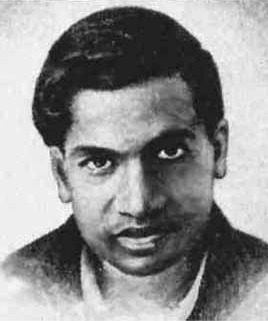
\includegraphics[width=2cm]{../Pictures/Ramanujan1915.jpg}
\end{minipage}
\newpage
\section{The Eisenstein series of weight $2$}
In this exercise we will study $G_2(z)$, which is \emph{not} a modular form for $\SL_2(\ZZ)$. Define $G_2(z)$ as
\[
G_2(z)= \sum_{n\neq 0} \frac 1{n^2} +\sum_{m\neq 0}\sum_{n\in\ZZ} \frac{1}{(mz+n)^2}.
\]
Note that we need to specify the order of summation because the series does not converge absolutely. You can use the formula, which has been proved in class:
\begin{equation}
\label{eq:G2}
G_2(-1/z) = z^2G_2(z)- 2\pi i z.
\end{equation}

\begin{enumerate}
\item Prove that $G_2$ satisfies $G_2(z+1)=G_2(z)$ and that it  has the $q$-expansion
\[
G_2(z) = 2\zeta(2) - 8\pi^2\sum_{n=1}^\infty \sigma_1(n)q^n,\quad q=e^{2\pi i z}.
\]
\item Deduce from~\ref{eq:G2} and part $1$ the transformation formula
\[
G_2(\gamma z) = (cz+d)^2G_2(z)- 2\pi i c(cz+d),\quad \gamma=\mtx abcd.
\]
\item Show that the non-holomorphic function  $G_2^*(z) = G_2(z)-\pi/\Im(z)$ is weight-$2$-invariant under $\SL_2(\ZZ)$.
\end{enumerate}

\section{A motivated proof of a formula seen in class}

The goal of this exercise is to prove the formula
\begin{equation}
\label{eq:cot}
\sum_{n\in\ZZ} \frac{1}{(z+n)^k} = \frac{(-2\pi i)^k}{(k-1)!}\sum_{m=1}^\infty m^{k-1}q^m,\quad k\geq 2, z\in\cH.
\end{equation}
without appealing to the cotangent function. Consider the function $f(z) = \sum_{n\in\ZZ} 1/(z+n)^k$, which is holomorphic on $\cH$ and is $1$-periodic. Let $f(z) = \sum_{m=1}^\infty a_m q^m = g(q)$ be its Fourier expansion (here $q = e^{2\pi i z}$).
\begin{enumerate}
\item Show that
\[
a_m = \frac{1}{2\pi i} \int_C\frac{g(q)}{q^{m+1}} dq,
\]
where $C$ is a contour that which traverses once counterclockwise a circle of radius $1$ about $0$.
\item Show that for any $y > 0$ we have
\[
a_m = \int_{iy}^{1+iy} f(z) e^{-2\pi i m z}dz = \int_{-\infty + iy}^{\infty + iy} z^{-k} e^{-2\pi i mz }dz.
\]
\item Consider the function $g_m(z) = z^{-k} e^{-2\pi i m z}$, which is a meromorphic function on $\CC$. Show that $g(z)$ is holomorphic on $\CC\setminus\{0\}$, and calculate $\operatorname{Res}_{z=0} g_m(z)$ by using the Taylor series of the exponential.
\item Prove the formula~\eqref{eq:cot} by applying the Residue theorem to the function $g_m$ and a large rectangular contour whose top side gives $a_m$.
\end{enumerate}
% Denote, for each $m\neq 0$, by $S_m(z)$ the quantity
% \[
% S_m(z)=\sum_{n\in \ZZ} \frac{1}{(mz+n)^2}.
% \]
% To show that $G_2(z+1)=G_2(z)$, we must show that
% \[
% \sum_{n\neq 0}\frac{1}{(m(z+1)+n)^2} = \sum_{n\neq 0} \frac{1}{(mz+n)^2}.
% \]
% This follows from the fact that the sum converges absolutely and $n\mapsto n+m$ is a bijection of $\ZZ$ (for each fixed $m\in\ZZ$).

% Next, we compute the $q$-expansion of $G_2$. This is done as we did in class. First, note that
% \[
% G_2(z)=2\zeta(2)+2\sum_{m=1}^\infty \sum_{n\in\ZZ}\frac{1}{(mz+n)^2}.
% \]
% Using now Lemma 1.4.5, with $z$ substituted by $mz$, we obtain
% \[
% G_2(z)=2\zeta(2)-8\pi\sum_{m=1}^\infty\sum_{d=1}^\infty dq^{md}.
% \]
% Grouping terms contributing to a given power of $q$ gives the formula.

% Part 2a is a direct calculation, by expanding $G_2(\gamma_1\gamma_2z)$, using the cocycle property of $j(\gamma,z)$ and calculating the lower left entry of the product of two matrices.

% Part 2b: substituting $-1/z$ in the definition we get:
% \[
% G_2(-1/z) = \sum_{n\neq 0} \frac 1{n^2} + \sum_{m\neq 0}\sum_{n\in\ZZ}\frac{z^2}{(mz-n)^2} = \sum_{n\neq 0} \frac 1{n^2} + \sum_{m\neq 0}\sum_{n\in\ZZ}\frac{z^2}{(m-nz)^2}
% \]
% This can be rewritten as
% \[
% 2\zeta(2) + z^2\left(\sum_{n\neq 0}\sum_{m\neq 0}\frac{1}{(mz+n)^2}\right)=2\zeta(2)+z^2\left(\sum_{n\neq 0}\sum_{m\neq 0} \frac{1}{(mz+n)^2} + 2\zeta(2)\right).
% \]
% The outer term $2\zeta(2)$ can be put into the sum corresponding to the term $n=0$, getting the desried formula.

% 2.c: the first identity follows from the partial fraction decomposition:
% \[
% \frac{1}{(mz+n)(mz+n+1)} = \frac{1}{mz+n}-\frac{1}{mz+n+1}.
% \]
% This implies that the inner sum telescopes to $0$, for each $m\neq 0$. Subtracting this series from the definition of $G_2(z)$ (which can be done term by term, this only needs conditional convergence) we get the new formula involving an absolutely convergent sum.

% 2.d: we compute from 2.b and 2.c:
% \[
% z^{-2}G_2(-1/z)-G_2(z) = \sum_{n\in\ZZ}\sum_{m\neq 0}\frac{1}{(mz+n)^2} - \sum_{m\neq 0,n\in\ZZ} \frac{1}{(mz+n)^2(mz+n+1)}.
% \]
% Subtracting term by term and using that
% \[
% \frac{1}{(mz+n)^2} - \frac{1}{(mz+n)^2(mz+n+1)} = \frac{1}{(mz+n)(mz+n+1)}
% \]
% gives the formula.

% 2.e: First, for each fixed $N$ we can reverse the sum and calculate, since the inner sum telescopes:
% \begin{align*}
% \sum_{m\neq 0}\sum_{n=-N}^{N-1} \left(\frac{1}{mz+n}-\frac{1}{mz+n+1}\right) &= \sum_{m\neq 0} \left(\frac{1}{mz-N} - \frac{1}{mz+N}\right)\\
% &=\frac{-1}{z}\sum_{m\neq 0}\left( \frac{1}{N/z + m}+\frac{1}{N/z-m}\right)\\
% &=\frac{-2\pi}{z}\cot(\pi N/z).
% \end{align*}
% Finally, taking the sum as $N\to \infty$ and using that
% \[
% \pi\cot(\pi N/z)=\pi i-2\pi i\sum_{m=0}^\infty e^{2\pi i mN/z}
% \]
% we get the formula.
\end{document}